\documentclass[load-preamble]{cnltx-doc}
\usepackage[T1]{fontenc}
\usepackage[utf8]{inputenc}

\usepackage{filecontents}

\usepackage{imakeidx}
\begin{filecontents*}{\jobname.ist}
 heading_prefix "{\\bfseries "
 heading_suffix "\\hfil}\\nopagebreak\n"
 headings_flag  1
 delim_0 "\\dotfill"
 delim_1 "\\dotfill"
 delim_2 "\\dotfill"
 delim_r "\\textendash"
 delim_t ""
 suffix_2p "\\nohyperpage{\\,f.}"
 suffix_3p "\\nohyperpage{\\,ff.}"
\end{filecontents*}
\indexsetup{othercode=\footnotesize}
\makeindex[options={-s \jobname.ist},intoc,columns=2,columnsep=1em]

\setcnltx{
  name     = cnltx ,
  title    = the cnltx bundle ,
  version  = \csname cnltx@@version\endcsname ,
  date     = \csname cnltx@@date\endcsname ,
  subtitle = Documentation for \LaTeXe\ Packages or Classes ,
  info     = \LaTeX\ examples the \texorpdfstring{\textsc{cn}}{CN} way ,
  authors  = Clemens Niederberger ,
  email    = contact@mychemistry.eu ,
  url      = https://github.com/cgnieder/cnltx ,
  abstract = {%
    A bundle of packages and classes for consistent format of control
    sequences, package options, source code with examples, writing a package
    manual (including an index containing the explained control sequences,
    options, \ldots).%
  } ,
  add-cmds = {
    cnltx@define@colorscheme,
    code,codefont,command,cs,csidx,
    darg,Default,default,
    env,environment,
    key,keybool,keychoice,keyval,
    marg,
    newarg,
    oarg,
    opt,option,
    sarg,setcnltx
  },
  add-envs = {
    commands,
    environments,
    example,
    options
  },
  add-frame-options = {
    innerleftmargin=2em
  }
}

\makeatletter
\def\cnltxbase{\cnltx@package@name@format{cnltx-base}}
\def\cnltxexample{\cnltx@package@name@format{cnltx-example}}
\def\cnltxcsnames{\cnltx@package@name@format{cnltx-csnames}}
\def\cnltxdoc{\cnltx@package@name@format{cnltx-doc}}

\newrobustcmd\bypackage{%
  \cnltx@version@note{provided by the \cnltxexample\ package}%
}
\newrobustcmd\byclass{%
  \cnltx@version@note{provided by the \cnltxdoc\ class}%
}
\makeatother

\newcommand*\file[1]{\code{#1}}

\newenvironment{colors}
  {%
    \def\colour##1{\item\code{\textcolor{##1}{##1}}}%
    \cnltxlist
  }
  {\endcnltxlist}

% \usepackage{showframe}
% \usepackage{kantlipsum}

\begin{document}

\section{Background}

The \cnltx\ bundle contains of different packages and classes.  I developed
them as a successor of a class that I used for writing the documentation of my
packages with the intention of a cleaner interface and less unnecessary
ballast.  Hence the separation into package and class.  The package provides a
source code environment that also prints the output and defines quite a number
of macros for formatting of control sequence names, package names, package
options and so on.  The best documentation for the bundle as always is the
source code but I'm trying to provide a documentation as comprehensive as
possible.

\section{Bundled Packages and Classes}

The \cnltx\ bundle currently bundles the following packages and classes:
\begin{itemize}
  \item \cnltxbase\ -- defines base macros for error-messaging, expansion
    control and tokenlist manipulation.  It also provides color definitions
    and defines a few color schemes for the \cnltxdoc\ class.  All other
    packages and classes of the cnbundle load this package.
  \item \cnltxexample\ -- defines macros and environments for describing
    control sequences and options and for including source code.
  \item \cnltxcsnames\ -- defines a list of highlighted control sequence
    names, loaded by \cnltxexample.
  \item \cnltxdoc\ -- a class for writing package manuals.  Loads
    \cnltxexample.
\end{itemize}

\section{License and Requirements}\label{sec:license}
\license

The \cnltxbase\ package loads the following packages:
\pkg{pgfopts}\footnote{\CTANurl{pgfopts}},
\pkg{etoolbox}\footnote{\CTANurl{etoolbox}},
\pkg{trimspaces}\footnote{\CTANurl{trimspaces}} and
\pkg{xcolor}\footnote{\CTANurl{xcolor}}.

The \cnltxexample\ package loads the following packages:
\cnltxbase, \pkg{listings}\footnote{\CTANurl{listings}},
\pkg{accsupp}\footnote{\CTANurl[macros/latex/contrib/oberdiek]{accsupp}},
\pkg{mdframed}\footnote{\CTANurl{mdframed}} and
\pkg{idxcmds}\footnote{\CTANurl{idxcmds}}.

The \cnltxdoc\ class loads the package with the same name and additionally
the following packages: \cnltxbase, \cnltxexample,
\pkg{ulem}\footnote{\CTANurl{ulem}},
\pkg{multicol}\footnote{\CTANurl[macros/latex/required/tools]{multicol}},
\pkg{ragged2e}\footnote{\CTANurl[macros/latex/contrib/ms]{ragged2e}},
\pkg{marginnote}\footnote{\CTANurl{marginnote}} and
\pkg{hyperref}\footnote{\CTANurl{hyperref}}. It is a wrapper class for the
\KOMAScript\ class \cls{scrartcl}\footnote{\CTANurl{koma-script}}.

Like all of my packages \cnltx\ implicitly relies on an up to date \TeX\
distribution.

\section{Options and Setup}
The \cnltx\ bundle has a number of options.  The \cnltxdoc\ class only knows
the \option{load-preamble} (described in section~\ref{sec:preamble}) as a
\emph{class} option.  All other options regardless if they're defined by a
package or a class can be set with a setup command:
\begin{commands}
  \command{setcnltx}[\marg{options}]
    setup command for \cnltx.
\end{commands}
The source code environments defined by the \cnltxexample\ package also have
optional arguments that can be used to set the options for the environment
locally.

\section{Available Commands}
\subsection{Description of Macros, Environments and  Options}\label{sec:cmds:macros}

The commands described in this section all are provided by the \cnltx\
package\bypackage.  They all are related to the typesetting of provided
macros, options and the like.

\begin{commands}
  \command{code}[\marg{arg}]
    Formatting of source code.  This is \emph{no} verbatim command.  Used
    internally in the following commands.
  \command{cs}[\sarg\marg{name}]
    Format the control sequence \meta{name}, \cs{cs}\code{\{name\}}:
    \cs*{name}.  Adds a corresponding index entry.  The starred form does not
    add an index entry.
  \command{csidx}[\marg{name}]
    Adds an index entry but does not typeset the control sequence
    \meta{name}.
  \command{env}[\sarg\marg{name}]
    Format the environment \meta{name}, \cs{env}\code{\{name\}}:
    \env*{name}.  Adds a corresponding index entry with a hint that the entry
    refers to an environment.  The starred form does not add an index entry.
  \command{envidx}[\marg{name}]
    Adds an index entry but does not typeset the environment \meta{name}.
  \command{meta}[\marg{meta}]
    Description of an argument, \cs{meta}\code{\{meta\}}: \meta{meta}.
  \command{marg}[\marg{arg}]
    A mandatory argument. \meta{arg} is formatted with \cs{meta} if it is not
    blank, \cs{marg}\code{\{arg\}}: \marg{arg}.
  \command{oarg}[\marg{arg}]
    An optional argument. \meta{arg} is formatted with \cs{meta} if it is not
    blank, \cs{oarg}\code{\{arg\}}: \oarg{arg}.
  \command{darg}[\marg{arg}]
    An argument with parentheses as delimiters. \meta{arg} is formatted with
    \cs{meta} if it is not blank, \cs{darg}\code{\{arg\}}: \darg{arg}.
  \command{sarg}
    An optional star argument, \cs{sarg}: \sarg.
  \command{option}[\sarg\marg{name}]
    An option \meta{name}, \cs{option}\code{\{name\}}: \option{name}.  Adds a
    corresponding index entry.  The starred form does not add an index entry.
  \command{optionidx}[\marg{name}]
    Adds an index entry but does not typeset the option \meta{name}.
  \command{key}[\sarg\marg{name}\marg{values}]
    A key \meta{name} with values \meta{values},
    \cs{key}\code{\{key\}}\code{\{value\}}: \key{key}{value};
    \cs{key}\sarg\code{\{key\}}\code{\{value\}}: \key*{key}{value}
  \command{choices}[\marg{clist of choices}]
    A list of choices, \cs{choices}\code{\{one,two,three\}}:
    \choices{one,two,three}
  \command{choicekey}[\marg{name}\marg{clist of choices}]
    A key \meta{name} with a list of possible values,
    \cs{choicekey}\code{\{key\}\{one,two,three\}}:
    \choicekey{key}{one,two,three}
  \command{boolkey}[\marg{name}]
    A boolean key \meta{name} with choices \code{true} and \code{false},
    \cs{boolkey}\code{\{key\}}: \boolkey{key}
  \command{default}[\marg{value}]
    Markup for a default choice,
    \cs{choices}\code{\{one,\cs{default}\{two\},three\}}:
    \choices{one,\default{two},three}
\end{commands}


\subsection{Versioning Commands, Licensing and Related  Stuff}\label{sec:cmds:versioning}

The commands described in this section are provided by the \cnltx\
class\byclass\ except where indicated differently.  These commands are related
to information about the legal stuff of a package and where to find it on th
world wide web.

\begin{commands}
  \command{sinceversion}[\marg{version}]
    \sinceversion{0.0}Gives a sidenote like the one on the left.
  \command{changedversion}[\marg{version}]
    \changedversion{0.0}Gives a sidenote like the one on the left.
  \command{lppl}
    Typesets ``\lppl'' and adds a corresponding index entry.
  \command{LPPL}
    Typesets ``\LPPL'' and adds a the same index entry as \cs{lppl}.
  \command{license}[\sarg]
    Typesets `\license*'.  The un-starred variant adds a \cs*{par}.
  \command{ctan}
    Typesets ``\ctan'' and adds a corresponding index entry.
  \command{CTAN}
    Typesets ``\CTAN'' and adds the same index entry as \cs{ctan}.
  \command{pkg}[\sarg\marg{package}]
    \bypackage Format the package name \meta{package} and add an index entry.
    The starred variant adds nothing to the index.
  \command{pkgidx}[\marg{package}]
    \bypackage Add an index entry for the package \meta{package}.
  \command{cls}[\sarg\marg{class}]
    \bypackage Format the class name \meta{class} and add an index entry.  The
    starred variant adds nothing to the index.
  \command{clsidx}[\marg{class}]
    \bypackage Add an index entry for the class \meta{class}.
  \command{CTANurl}[\oarg[directory]\marg{name}]
    Writes a \ctan\ link like the ones in section~\ref{sec:license} in the
    footnotes.  The predefined directory is \code{macros/latex/contrib}.
\end{commands}

\subsection{Formatting Commands}\label{sec:cmds:formatting}

One of the goals I wanted to achieve with this package is a consistent look
and an easy interface for customization.  No font choice and no color choice
is fixed.  In this section ways to change the formatting are shown.

The formatting of the different commands provided by \cnltx\ can be
changed in two ways: either by redefining the internal commands that are used
for the formatting or by setting a corresponding option.  Both variants are
described in the next subsections.

How the colors should be changed is described in section~\ref{sec:colors}.

\subsubsection{Formatting by Redefining Hooks}

You can change the formatting by redefining the following commands.  They're
all defined by the \cnltx\ package except where indicated differently.

\begin{commands}
  \command{codefont}\Default{\cs*{ttfamily}}
    This command is used for all formatting of source code.
  \command{sourceformat}\Default{\cs{codefont}\cs*{small}}
    Formatting of the listings.
  \command{exampleformat}\Default
    Special formatting of the output of a listing.
  \command{versionnoteformat}\Default{\cs*{footnotesize}\cs*{sffamily}\cs*{RaggedRight}}
    \byclass Formatting of the notes introduced in section~\ref{sec:cmds:versioning}.
  \command{packageformat}\Default{\cs*{sffamily}}
    The formatting of package names.
  \command{classformat}\Default{\cs*{sffamily}}
    The formatting of class names.
  \command{argumentformat}\Default{\cs*{normalfont}\cs*{itshape}}
    The formatting of \cs{meta}\marg{meta}.
\end{commands}

\begin{example}
  \renewcommand*\codefont{\sffamily\bfseries}
  \code{foo} and \cs*{bar}, option \option{baz}
\end{example}

\subsubsection{Formatting by Setting Options}

You can change the formatting by setting the following options.  They're all
defined by the \cnltx\ package except where indicated differently.

\begin{options}
  \keyval{code-font}{definition}\Default{\cs*{ttfamily}}
    Used for all formatting of source code.
  \keyval{source-format}{definition}\Default{\cs{codefont}\cs*{small}}
    Formatting of the listings.
  \keyval{expl-format}{definition}\Default
    Special formatting of the output of a listing.
  \keyval{version-note-format}{definition}%
  \Default{\cs*{footnotesize}\cs*{sffamily}\cs*{RaggedRight}}
    \byclass Formatting of the notes introduced in
    section~\ref{sec:cmds:versioning}.
  \keyval{pkg-format}{definition}\Default{\cs*{sffamily}}
    The formatting of package names.
  \keyval{cls-format}{definition}\Default{\cs*{sffamily}}
    The formatting of class names.
  \keyval{arg-format}{definition}\Default{\cs*{normalfont}\cs*{itshape}}
    The formatting of \cs{meta}\marg{meta}.
\end{options}

\begin{example}
  \setcnltx{code-font=\sffamily\itshape}
  \code{foo} and \cs*{bar}, option \option{baz}
\end{example}

\section{Available Environments}\label{sec:envs}

\cnltx\ defines a few environments most of them related to the way how
descriptions of commands are typeset.

The \env{example} environment is defined by the \cnltx\ package, the
others are defined by the class.

\begin{environments}
  \environment{example}[\oarg{options}]
    This environment is a formatted verbatim environment that also inputs the
    output of the inputted code.  This environment is described in
    section~\ref{sec:usage:examples}.
  \environment{sourcecode}[\oarg{options}]
    This environment is a formatted verbatim environment.  This environment is
    described in section~\ref{sec:usage:examples}.
  \environment{commands}
    A description-like environment for describing commands.  While this
    environment is a list internally and thus recognizes \cs*{item} own
    commands are used to describe macros.  They are explained in
    section~\ref{sec:usage:commands}.
  \environment{options}
    A description-like environment for describing options.  While this
    environment is a list internally and thus recognizes \cs*{item} own
    commands are used to describe options.  They are explained in
    section~\ref{sec:usage:options}.
  \environment{environments}
    A description-like environment for describing environments.  While this
    environment is a list internally and thus recognizes \cs*{item} own
    commands are used to describe environments.  They are explained in
    section~\ref{sec:usage:environments}.
\end{environments}

Except for the \env{example} and the \env{sourcecode} environments the
environments are lists all using the same internal \cs*{list}.  The setup uf
this list can be changed via an option:

\begin{options}
  \keyval{list-setup}{definitions}{}
    \Default{\cs*{leftmargin}=0pt \cs*{labelwidth}=2em \cs*{labelsep}=0pt
      \cs*{itemindent}=-1em }
    The setup of the \cs*{list} used by the \env{commands}, \env{options} and
    \env{environments} environments.
\end{options}

\section{Usage}
\subsection{Command Descriptions}\label{sec:usage:commands}
Inside of the environment \env{commands} that was introduced in
section~\ref{sec:envs} items are input via the following command:
\begin{commands}
  \command{command}[\sarg\marg{name}\oarg{stuff after}]
    This macro formats a control sequence with \cs{cs} and puts a line break
    after it.  The optional argument allows printing things directly after the
    command name and can thus be used for adding arguments.
  \command{Default}[\marg{code}]
    This command can be placed after \cs{command} in order to give a default
    definition.  The definition will then be placed on the same line flush
    right.
\end{commands}
\begin{example}
  \begin{commands}
    \command{cs}
      This is about foo bar baz.
    \command{cs}[\marg{arg}]
      This one has an argument.
    \command{cs}[\sarg\oarg{option}]
      This has a star variant and an optional argument.
    \command{cs}\Default{foo bar}
      This one has the default replacement text \code{foo bar}
  \end{commands}
\end{example}

\subsection{Option Descriptions}\label{sec:usage:options}

The \env{options} environment knows a few more commands to meet all the
different kinds of options.
\begin{commands}
  \command{opt}[\sarg]
    An option.  The star prevents an index entry.
  \command{keyval}[\sarg\marg{key}\marg{value}]
    A key/value option.  The star prevents an index entry.
  \command{keychoice}[\sarg\marg{key}\marg{list of choices}]
    A key/value option where the value is one of a list of choices.  The star
    prevents an index entry.
  \command{keybool}[\sarg\marg{name}]
    A boolean key, that ist a choice key with choices \code{true} and 
    \code{false}.  The star prevents an index entry.
\end{commands}

\begin{example}
  \begin{options}
    \opt{foo}
      This makes stuff.  Let's add a few more words so that the line gets
      filled and we can see how the output actually looks.
    \opt*{foo}\Default{bar}
      This makes stuff.  Let's add a few more words so that the line gets
      filled and we can see how the output actually looks.
    \keyval{foo}{bar}\Default
      This makes stuff.  Let's add a few more words so that the line gets
      filled and we can see how the output actually looks.
    \keyval*{foo}{bar}
      This makes stuff.  Let's add a few more words so that the line gets
      filled and we can see how the output actually looks.
    \keychoice{foo}{one,two,three}
      This makes stuff.  Let's add a few more words so that the line gets
      filled and we can see how the output actually looks.
    \keybool{foo}
      This makes stuff.  Let's add a few more words so that the line gets
      filled and we can see how the output actually looks.
  \end{options}
\end{example}

\subsection{Environment Descriptions}\label{sec:usage:environments}

Environment descriptions are made -- unsurprisingly -- with the
\env{environments} environment.  It knows the command \cs{environment}:

\begin{commands}
  \command{environment}[\sarg\marg{name}\oarg{stuff after}]
    This macro prints the environment name and puts a line break
    after it.  The optional argument allows printing things directly after the
    environment name and can thus be used for adding arguments.
\end{commands}

\begin{example}
  \begin{environments}
    \environment*{foobar}[\oarg{options}]
      This is environment \env*{foobar}.  The star prevents it from being
      added to the index.
  \end{environments}
\end{example}

\subsection{Example Code}\label{sec:usage:examples}

Example code can be included through the \env{example} environment or the
\env{sourcecode} environment.
\begin{sourcecode}
  \begin{example}
    a \LaTeX\ code example
  \end{example}
\end{sourcecode}
This example would give:

\begin{example}
  a \LaTeX\ code example
\end{example}

Both environments can be influenced by options:
\begin{options}
  \keybool{code-only}\Default{false}
    Only typeset the code as code but don't include it afterwards.  The
    code box above is an example for the usage of this option.  This option
    has no effect on the \env{sourcecode} environment: this is already what
    that environment does.
  \keybool{side-by-side}\Default{false}
    Typeset source and output side by side.  The code is input on the left and
    the output on the right.  Side by side examples are typeset in
    \env*{minipage} environments with all consequences that come with them
    (think of \cs*{parindent} \ldots).
  \keyval{code-sep}{definition}\Default{\cs*{hrulefill}}
    Code that is inserted between a source code and the corresponding output
    when printed below each other.
\end{options}

The same example again, this time using \option{side-by-side}:

\begin{example}[side-by-side]
  a \LaTeX\ code example
\end{example}

The frame around the examples is done by the \pkg{mdframed} package.  It is of
course possible to customize it:
\begin{options}
  \keyval{add-frame-options}{\pkg{mdframed} options}\Default
    Add options to the predefined ones.
  \keyval{frame-options}{\pkg{mdframed} options}{}
    \Default{backgroundcolor=cnltxbg,linecolor=cnltx,roundcorner=5pt}
    Overwrite the options with new ones.
\end{options}

The source code is formatted using the \pkg{listings} package.  Similar
options exist to adapt \pkg{listings}' options that are used for formatting
the source code.  The predifined style has many options that will not be
mentioned here.  If you're interested you can find them in
\file{cnltx-csnames.sty}.
\begin{options}
  \keyval{gobble}{integer}\Default{2}
    The number of initial characters that is gobbled from each line.
  \keyval{add-cmds}{list of csnames}\Default
    A list of control sequence names that should be recognized as a command
    sequence in the source code examples and should be formatted accordingly.
    The control sequence names in this list will also get an index entry when
    they're used in the source example.  This is done internally via
    \cs{csidx}.  The option should be used to add the new commands that are
    defined by the package for which you are writing the manual for.
  \keyval{add-silent-cmds}{list of csnames}
    A list of control sequence names that should be recognized as a command
    sequence in the source code examples and should be formatted accordingly.
    The control sequence names in this list will \emph{not} get an index entry
    when they're used in the source example.  There already is quite a large
    but far from comprehensive list of silent commands but many are still
    missing.  This option allows you to extend the list on a per document
    basis.
  \keyval{add-listings-options}{\pkg{listings} options}\Default
    Additional options for the \pkg{listings} environments.
  \keyval{listings-options}{\pkg{listings} options}
    Overwrite existing options with new ones.  This can be used to build an own
    style from scratch.
  \keyval{add-envs}{list of environment names}\Default
    Like \option{add-cmds} but for environment names.
\end{options}


  
\section{Package or Class Information,  Building of the Manuals Title Page}
\subsection{Package or Class Information}

A manual for a package or a class needs some information like the package
name, the version number, the date and so on.  This information is given with
the following options.  They are used to build the title page of the manual.
\begin{options}
  \keyval{package}{package}
    The name of the package that is described.  Either this option or
    \option{class} or \option{name} should always be given.  This command also
    defines a command sequence from the package name that formats the package
    name with color and small caps like \cnltx.
  \keyval{class}{class}
    The name of the class that is described.  Either this option or
    \option{package} or \option{name} should always be given.  This command
    also defines a command sequence from the class name that formats the class
    name with color and small caps like \cnltx.
  \keyval{name}{name}
    The name of the class/package that is described.  Either this option or
    \option{package} or \option{class} should always be given.  This command
    also defines a command sequence from the class name that formats the class
    name with color and small caps like \cnltx.
  \keyval{authors}{author list}
    Comma separated list of package/class authors.
  \keyval{version}{version number}
    Version number of the package/class.  \cnltx\ tries to extract the
    information from the given \option{package} or \option{class}.  This
    option can be used to set it explicitly.
  \keyval{date}{date}
    Date of the package/class.  \cnltx\ tries to extract the
    information from the given \option{package} or \option{class}.  This
    option can be used to set it explicitly.
  \keyval{info}{package/class info}
    Information about the package/class.  \cnltx\ tries to extract the
    information from the given \option{package} or \option{class}.  This
    option can be used to set it explicitly.
  \keyval{subtitle}{subtitle}
    A subtitle that is typeset \emph{instead} of the package/class info.
  \keyval{url}{url}
    The homepage of the package.
  \keyval{email}{email}
    A contact email address.
  \keyval{abstract}{abstract}
    An abstract of the package/class/manual.  This is text typeset in a box of
    \code{.75\cs*{linewidth}}.  Actually it does not have to be text but could
      be an image or whatever you like.
\end{options}

\subsection{Building of the Manuals Title Page}

If either the \option{package} or \option{class} has been given an automatic
title page is built using the gathered information. Figure~\ref{fig:titlepage}
roughly sketches which informations is used and how the different elements are
arranged on the title page.  The page style of the title page is
\code{plain}.  Additionally a  table of contents is automatically built that
is set in two columns.

\begin{figure}[htb]
  \centering
  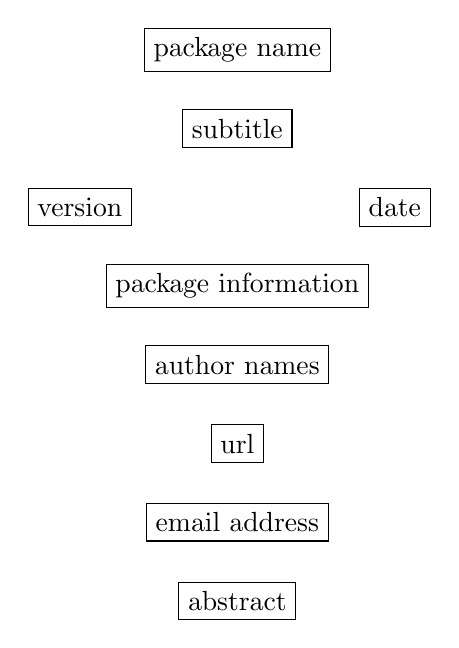
\begin{tikzpicture}
    \node[draw] at (0,0) {package name} ;
    \node[draw] at (0,-1) {subtitle} ;
    \node[draw] at (-2,-2) {version} ;
    \node[draw] at (2,-2) {date} ;
    \node[draw] at (0,-3) {package information} ;
    \node[draw] at (0,-4) {author names} ;
    \node[draw] at (0,-5) {url} ;
    \node[draw] at (0,-6) {email address} ;
    \node[draw] at (0,-7) {abstract} ;
  \end{tikzpicture}
  \caption{Schematic sketch of the title page.}
  \label{fig:titlepage}
\end{figure}

\subsection{Predefined Preamble}\label{sec:preamble}

It is posssible to load a part of my standard preamble automatically by
passing an option as class option.
\begin{options}
  \opt{load-preamble}
    Class option that preloads part of my custom preamble.
\end{options}

Using the option will include the following code:

\begin{sourcecode}
  \RequirePackage[oldstyle]{libertine}
  \RequirePackage{libertinehologopatch}% not on CTAN, yet!
  \RequirePackage[supstfm=libertinesups]{superiors}
  \RequirePackage{microtype}
  \RequirePackage[scaled=.83]{beramono}
  \RequirePackage{fnpct}
  \RequirePackage[english]{babel}
  \renewcommand*\othersectionlevelsformat[3]{%
    \textcolor{cnltx}{#3\autodot}\enskip}
  \renewcommand*\partformat{%
    \textcolor{cnltx}{\partname~\thepart\autodot}}
  \deffootnote{2em}{1em}{\llap{\thefootnotemark. }}%
  \pagestyle{headings}
  \setcapindent{1.5em}
  \setkomafont{caption}{\normalfont\footnotesize\sffamily}
  \setkomafont{captionlabel}{\normalfont\footnotesize\sffamily\scshape}
\end{sourcecode}

\section{Predefined Colors and Color-Schemes}\label{sec:colors}
\subsection{Explicitly Defined Colors}\label{sec:colors:definitions}

The \cnltxbase\ package defines a number of colors:
\begin{colors}
  \colour{cnltxbrown}
    Per default used for the control sequences.
  \colour{cnltxblue}
    Unused per default.
  \colour{cnltxred}
    Per default used as base color in various places.
  \colour{cnltxgreen}
    Unused per default.
  \colour{cnltxgray}
    Per default used for formatting comments.
  \colour{cnltxyellow}
    Per default used for options.
  \colour{cnltxformalblue}
    Unused per default.
  \colour{cnltxformalred}
    Unused per default.
\end{colors}

\subsection{Actual Used Color Names and Color Schemes}

The colors defined in section~\ref{sec:colors:definitions} are not directly
used with those names.  Instead colors are used whose names describe their
function rather than the color.  For this the color names are mapped to actual
colors and saved as a coloring scheme.  There are currently three predefined
color schemes whose definitions are given below.  Those definitions also show
the actually used color names:

The `default' color scheme is defined as follows:
\begin{sourcecode}
  \cnltx@define@colorscheme{default}{
    cs          => cnltxbrown , % command sequences
    option      => cnltxyellow ,% options
    comment     => cnltxgray ,  % comments
    beginend    => red ,        % \begin and \end
    env         => black ,      % environment names
    argument    => black ,      % argument delimiters
    meta        => black!80 ,   % arguments of \meta
    cnltx       => cnltxred ,   % base color
    cnltxbg     => white ,      % source code box background
    link        => black!90 ,   % hyperlinks
    versionnote => black!75     % versioning notes text 
  }
\end{sourcecode}

The `blue' color scheme is defined this way:
\begin{sourcecode}
  \cnltx@define@colorscheme{blue}{
    cs          => cnltxbrown ,
    option      => cnltxgreen ,
    comment     => cnltxgray ,
    beginend    => red ,
    env         => black ,
    argument    => black ,
    meta        => black!80 ,
    cnltx       => cnltxblue ,
    cnltxbg     => yellow!10 ,
    link        => cnltx ,
    versionnote => black!75
  }
\end{sourcecode}

Finally the `formal' color scheme is defined like this:
\begin{sourcecode}
  \cnltx@define@colorscheme{formal}{
    cs          => black ,
    option      => cnltxformalblue ,
    comment     => cnltxgray ,
    beginend    => red ,
    env         => black ,
    argument    => black ,
    meta        => black!80 ,
    cnltx       => cnltxformalblue ,
    cnltxbg     => white ,
    link        => black!90 ,
    versionnote => black!75
  }
\end{sourcecode}

\section{Internal Helper Commands}

The commands in this section are only described for the sake of completeness.
They are not meant to be used in a document.

\subsection{Defined by \cnltxbase}

Especially \cnltxbase\ defines some useful helper macros that are also used by
the other packages and classes.

\begin{commands}
  \command{cnltx\at\at date}
    The creation date of the current version of the bundle.
  \command{cnltx\at\at version}
    The version number of the bundle.
  \command{cnltx\at\at info}
    The short description of the bundle.
  \command{cnltx\at create\at message}%
    [\marg{module}\code{\{\choices{Error,Warning,WarningNoLine,Info}\}}]
    Create suiting error and warning messaging commands for the module
    \meta{module}.
  \command{cnltx\at base\at error}[\marg{message}]
    Issue an error message using \cs*{PackageError}.
  \command{cnltx\at base\at warning}[\marg{message}]
    Issue a warning message using \cs*{PackageWarning}.
    \command{cnltx\at base\at warningnoline}[\marg{message}]
    Issue a warning message using \cs*{PackageWarningNoLine}.
  \command{cnltx\at base\at info}[\marg{message}]
    Issue a message using \cs*{PackageInfo}.
  \command{cnltx\at fullexpand\at onearg}[\marg{cs}\marg{argument}]
    Exhaustive expansion of \meta{argument} before it is passed as argument to
    \meta{cs}.
  \command{cnltx\at fullexpand\at twoargs}[\marg{cs}\marg{argument1}\marg{argument2}]
    Exhaustive expansion of \meta{argument1} and \meta{argument2} before
    they're passed as argumenst to \meta{cs}.
  \command{cnltx\at stripbs}
    A shortcut for \lstinline[style=cnltx]+\expandafter\@gobble\string+.
  \command{cnltx\at if\at in}[\marg{tokenlist}\marg{search}\marg{true}\marg{false}]
    Places \meta{true} in the input stream if \meta{search} is found in
    \meta{tokenlist} and \meta{false} if it isn't.
  \command{cnltx\at replace\at once}[\marg{cs}\marg{search}\marg{replace}]
    Replaces the first occurence of \meta{search} in the first expansion of
    \meta{cs} with \meta{replace}.
  \command{cnltx\at replace\at all}[\marg{cs}\marg{search}\marg{replace}]
    Replaces all occurences of \meta{search} in the first expansion of
    \meta{cs} with \meta{replace}.
  \command{cnltx\at define\at colorscheme}[\marg{name}\marg{scheme definition}]
    Command that can be used to define a color scheme.
\end{commands}

\subsection{Defined by \cnltxexample}

\begin{commands}
  \command{cnltx\at example\at error}[\marg{message}]
    Issue an error message using \cs*{PackageError}.
  \command{cnltx\at example\at warning}[\marg{message}]
    Issue a warning message using \cs*{PackageWarning}.
    \command{cnltx\at example\at warningnoline}[\marg{message}]
    Issue a warning message using \cs*{PackageWarningNoLine}.
  \command{cnltx\at example\at info}[\marg{message}]
    Issue a message using \cs*{PackageInfo}.
  \command{at}
    Robust command that typesets `\at'.  An @ in command names confuses the
    indexing of the command names.  Either one uses another symbol for
    makeindex's ``actual'' recognition and also tells \pkg{idxcmds} about it
    or one uses \cs{at} in \cs{cs} and friends.
  \command{bang}
    Robust command that typesets `\bang'.
  \command{equal}
    Robust command that typesets `\equal'.
  \command{cnltx\at equal}
    Used in definitions of the key/value option typesetting commands.
  \command{indexcs}
    Version of \cs{csidx} that takes care of a \cs*{textcompwordmark} inserted
    by listings. Also replaces all occurences of @ with category code 11 or 12
    with \cs{at}. Used to index commands in the \env{sourcecode} and
    \env{example} environments that have been added with \option{add-cmds}.
  \command{newarg}[\marg{cs}\marg{left delim}\marg{right delim}]
    Command used to define the argument commands:
    \lstinline[style=cnltx]+\newarg\marg{\{}{\}}+
  \command{MakePercentComment}
    Sets the category code of \code{\%} to 14.
  \command{cnltx\at copyablespace}
    Prints a space that is also copyable.  Uses the \pkg{accsupp}.
  \command{cnltx\at mdframed\at options}
    Predefined option list for the \pkg{mdframed} style \code{cnltx}.
  \command{cnltx\at listings\at style}
    Predefined option list for the \pkg{listings} style \code{cnltx}.
\end{commands}

\subsection{Defined by \cnltxdoc}

\begin{commands}
  \command{cnltx\at doc\at error}[\marg{message}]
    Issue an error message using \cs*{PackageError}.
  \command{cnltx\at doc\at warning}[\marg{message}]
    Issue a warning message using \cs*{PackageWarning}.
    \command{cnltx\at doc\at warningnoline}[\marg{message}]
    Issue a warning message using \cs*{PackageWarningNoLine}.
  \command{cnltx\at doc\at info}[\marg{message}]
    Issue a message using \cs*{PackageInfo}.
  \command{cnltx\at getfileinfo}[\marg{file name}\marg{file extension}]
    Extract the date, version and background information for a package or a
    class.
  \command{cnltx\at newname}[\marg{cs}\marg{first name}{last name}]
    Defines \meta{cs} to write out the name and add an index entry.  Also
    defines a starred variant that only writes the last name but still adds an
    index entry.
  \command{cnltx\at version\at note}[\marg{note}]
    Command that is used for the versioning notes interally.  Sets
    \cs*{reversemarginpar} and then writes the note \meta{note} to the margin
    with corresponding formatting.
\end{commands}
\begin{environments}
  \environment{cnltxlist}
    The list environment that is used by the environments \env{commands},
    \env{options} and \env{environments}.
\end{environments}

\subsection{Defined by \cnltxcsnames}

\begin{commands}
  \command{cnltx\at predefined\at control\at sequences}
    A comma-separated list of predefind `silent' control sequence names.
\end{commands}

\printindex

\end{document}
